\section{Metodologija}

\begin{frame}
    \frametitle{Transformacije i evaluacija modela}

    \begin{columns}[T, totalwidth=\textwidth]

        % Leva kolona: transformacije
        \begin{column}{0.48\textwidth}
            \textbf{Transformacije:}

            \begin{itemize}
                \item \textbf{Log transformacija:} $y = \log(1 + x/30)$
                \begin{figure}
                    \centering
                    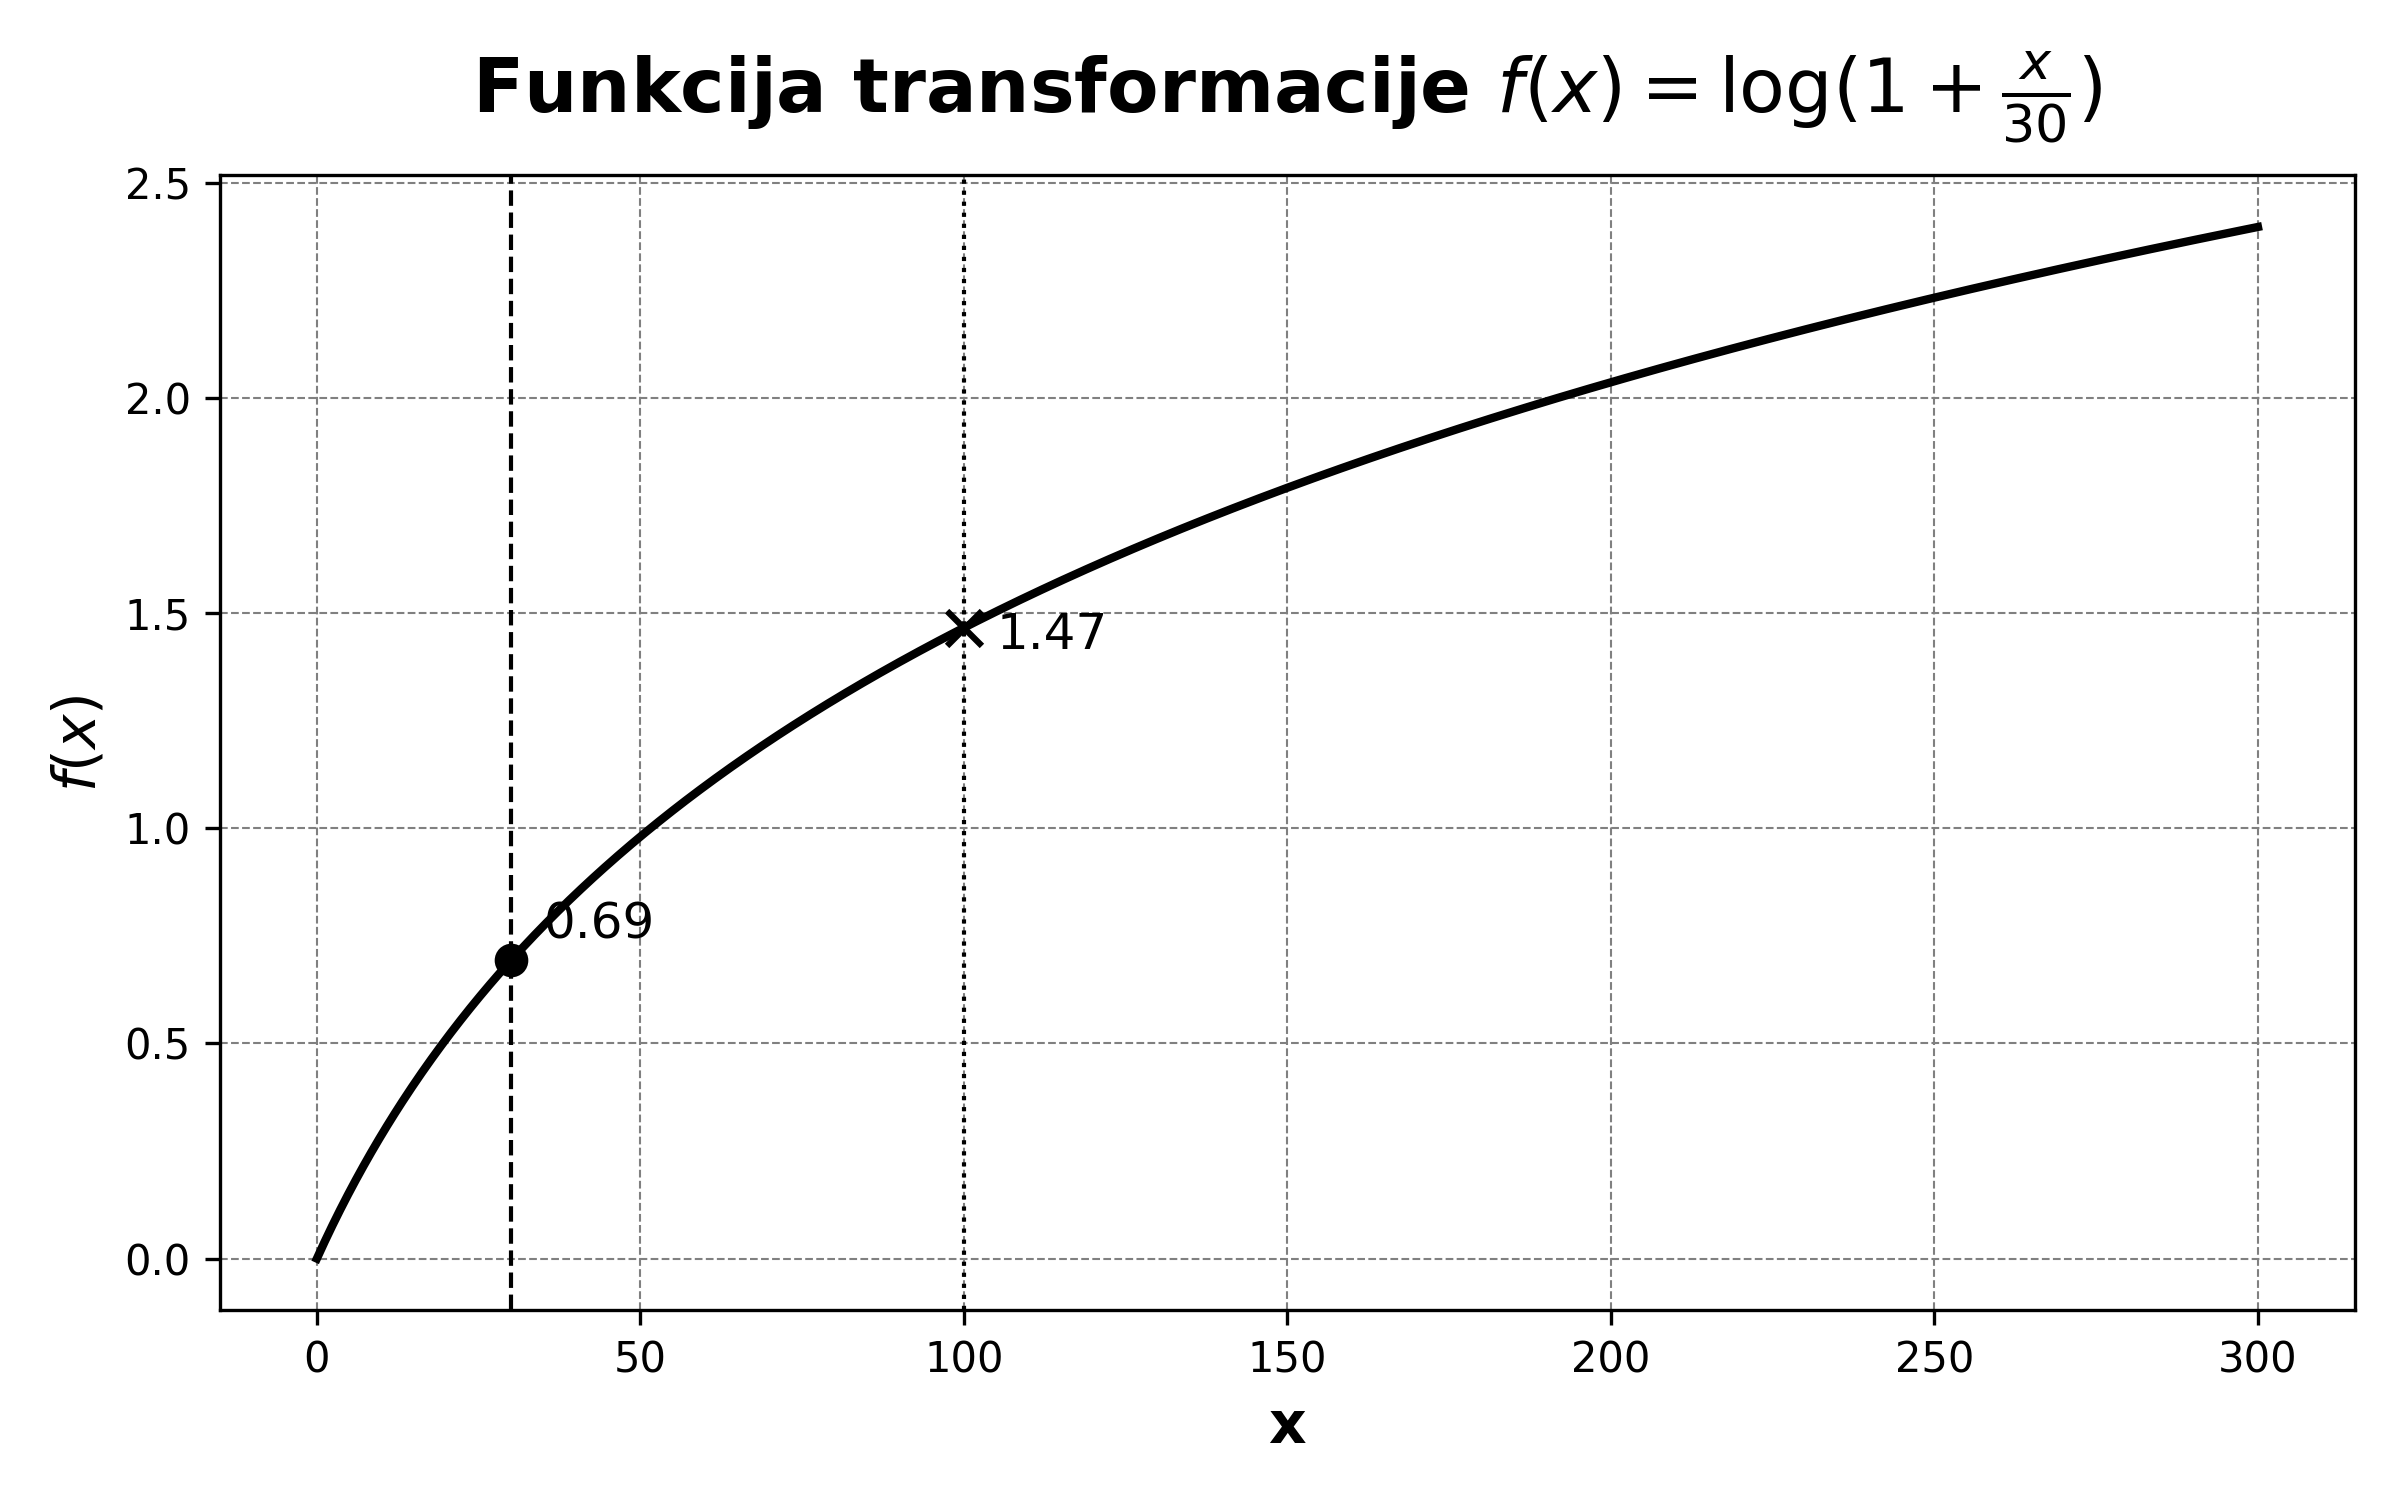
\includegraphics[width=0.75\textwidth]{images/log1p.png}
                \end{figure}

                \item \textbf{Box-Cox transformacija:} 
                {\small
                \[
                y = 
                \begin{cases} 
                \dfrac{x^\lambda - 1}{\lambda}, & \lambda \neq 0 \\
                \log(x), & \lambda = 0
                \end{cases}
                \]
                }
            \end{itemize}
        \end{column}

        % Desna kolona: evaluacija
        \begin{column}{0.48\textwidth}
            \textbf{Evaluacija: RMSLE}
            {\small
            \[
            \text{RMSLE} = \sqrt{\frac{1}{n}\sum_{i=1}^n \left( \log(1 + \hat{y}_i/30) - \log(1 + y_i/30) \right)^2}
            \]
            }

            \begin{itemize}
                \item $n$ -- broj primera u skupu podataka
                \item $y_i$ -- stvarna koncentracija polena za $i$-ti primer
                \item $\hat{y}_i$ -- predviđena koncentracija polena za $i$-ti primer
            \end{itemize}
        \end{column}

    \end{columns}

\end{frame}



\begin{frame}
    \frametitle{Efekat transformacija na koncentraciju polena}

    \begin{figure}
        \centering
        \includegraphics[width=\textwidth]{images/AMBROZIJA_POŽAREVAC_seasonal_concentration_transforms.png}

    \end{figure}
\end{frame}



\begin{frame}
    \frametitle{Imputacija podataka}

    \begin{figure}
        \centering
        \includegraphics[width=0.85\textwidth]{images/AMBROZIJA_POŽAREVAC_seasonal_decomposition.png}
        \caption{Signal nakon uklanjanja trenda}
    \end{figure}

\end{frame}




\begin{frame}
    \frametitle{Kriging i prostorno-vremenski variogram}

    \begin{columns}[T, totalwidth=\textwidth]

        % Leva kolona: slika
        \begin{column}{0.55\textwidth}
            \begin{figure}
                \centering
            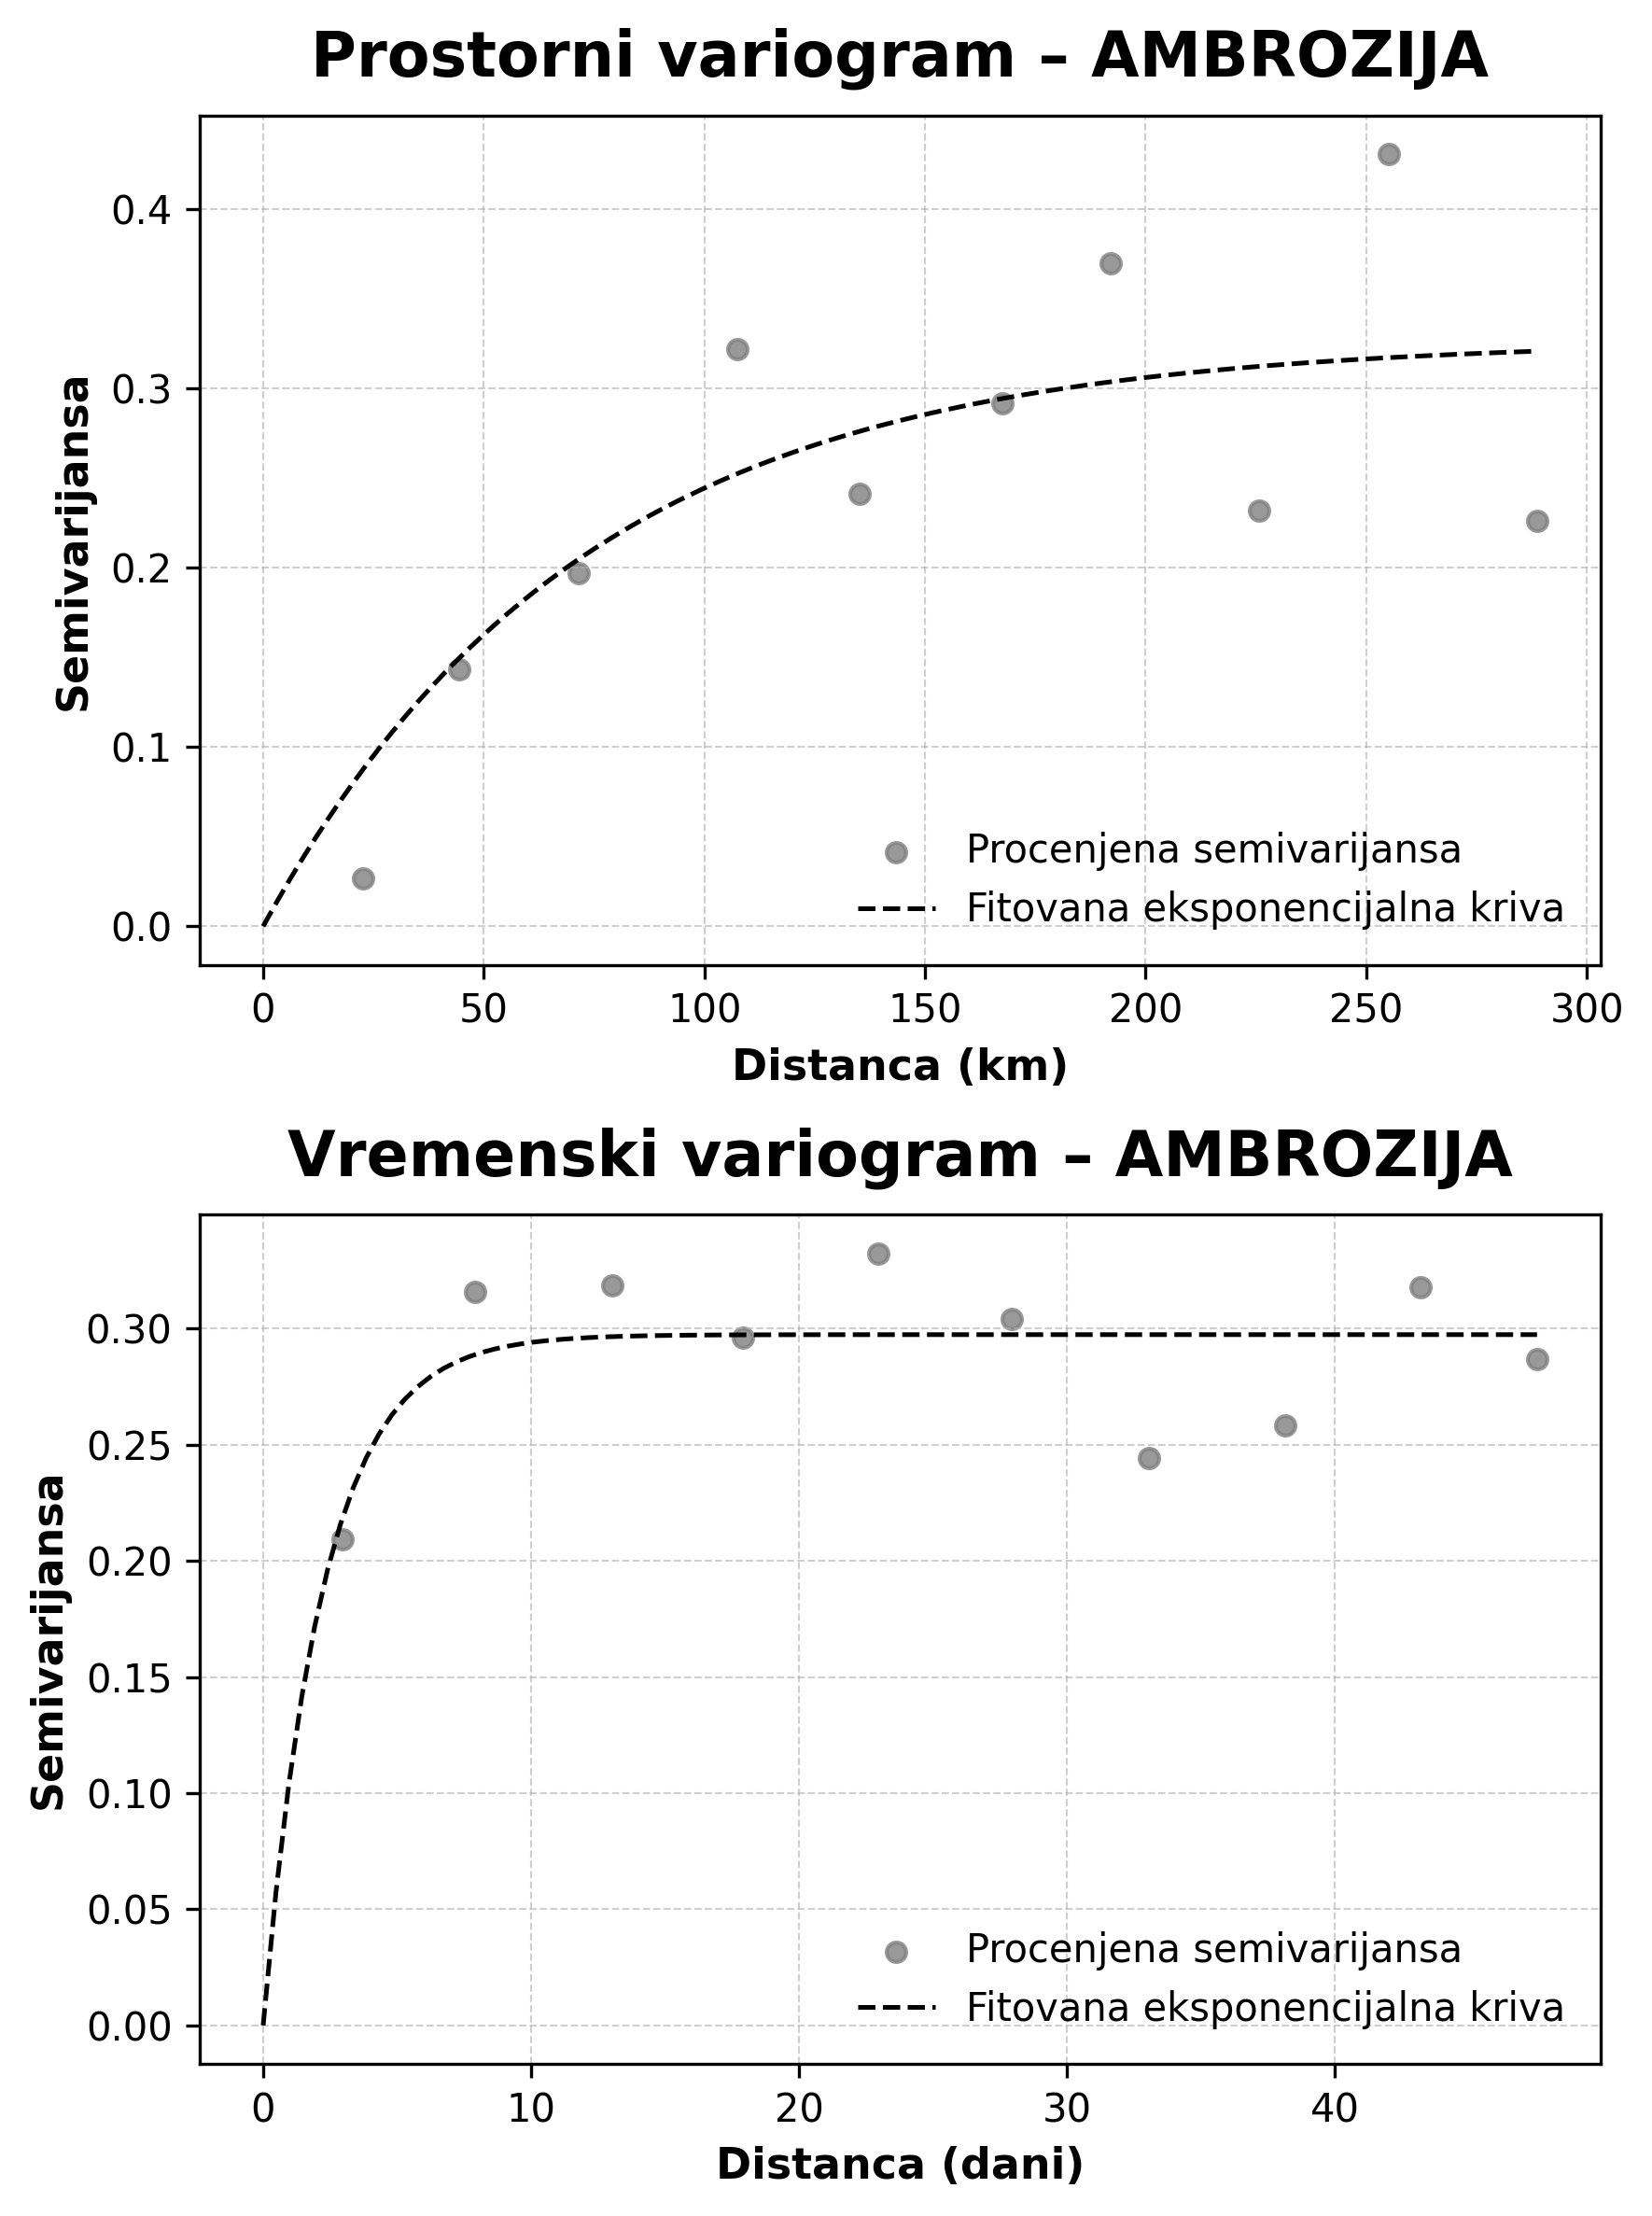
\includegraphics[height=0.9\textheight]{images/AMBROZIJA_variogrami.png}
            \end{figure}
        \end{column}

        % Desna kolona: tekst i formula
        \begin{column}{0.43\textwidth}
            Na osnovu dobijenih prostornog i vremenskog variograma, zajednički (prostorno-vremenski)
            variogram određen je prema sledećoj formuli:

            {\small
            \[
            \gamma(u, v) = \gamma(u, 0) + \gamma(0, v) - k \, \gamma(u, 0)\gamma(0, v)
            \]
            }

            gde je: 
            \begin{itemize}
                \item $\gamma(u, 0)$ -- prostorni variogram
                \item $\gamma(0, v)$ -- vremenski variogram
                \item $k$ -- parametar određen optimizacijom za najbolje zadovoljenje uslova separabilnosti
            \end{itemize}

        \end{column}

    \end{columns}

\end{frame}


\begin{frame}
    \frametitle{Modelovanje vremenskih serija: SARIMAX i Prophet}

    \begin{itemize}
        \item \textbf{SARIMAX} — sezonski ARIMA model sa egzogenim promenljivama \\
        Definisan parametrima \((p, d, q) \times (P, D, Q, s)\):
        {\small
        \[
        \Phi_P(L^s)\phi_p(L)(1 - L)^d(1 - L^s)^D y_t =
        \Theta_Q(L^s)\theta_q(L)\varepsilon_t + \beta^{T} \mathbf{x}_t 
        \]
        }
        gde su:
        \begin{itemize}
            \small{
            \item \(\phi_p(L)\), \(\theta_q(L)\) — AR i MA operatori
            \item \(\Phi_P(L^s)\), \(\Theta_Q(L^s)\) — sezonski AR i MA operatori
            \item \(d, D\) — red diferenciranja
            \item \(s\) — dužina sezonskog perioda
            \item \(\mathbf{x}_t\) — egzogene promenljive}
        \end{itemize}

        \vspace{0.2cm}
    \item \textbf{Prophet} — model razvijen od strane kompanije \textit{Meta} (bivši \textit{Facebook}), 
    pri čemu je u ovom radu primenjena njegova \textbf{multiplikativna varijanta}:   
        \[
        y(t) = g(t) \times (1 + s(t)) + \varepsilon_t
        \]
        gde su: \(g(t)\) — trend, \(s(t)\) — sezonska komponenta (Furijeovi redovi).
    \end{itemize}
\end{frame}


\begin{frame}
    \frametitle{Modelovanje vremenskih serija pomoću Random Foresta}

    \begin{itemize}
        \item Model baziran na \textbf{atributima izvedenim iz vremenskih serija}:
        \begin{itemize}
            \item Vrednosti koncentracije polena sa zaostatkom od nekoliko dana
            \item Prosečna koncentracija u prethodnih 7 dana
            \item Prosečna koncentracija u istom periodu prethodne godine (± 3 dana)
            \item Koncentracija na isti dan prethodne godine
            \item Broj dana od početka sezone i godina
            \item Furijeovi redovi za modelovanje sezonalnosti
        \end{itemize}

        \vspace{0.3cm}
        \item Ovim pristupom model ne koristi vremensku zavisnost direktno, već model uči obrasce iz generisanih vremenskih karakteristika.
    \end{itemize}
\end{frame}
